\chapter{Part 4b. Instruction Level Parallelism Basic Pipelining}
\section{Circuit Timing and Performance}

Most of the time, we have discussed circuits at a higher level of timing abstraction, focusing on what happens during each cycle:
\begin{itemize}
    \item[-] \textbf{Finite State Machines:} $\texttt{state} \gets \texttt{next\_state}$
    \item[-] \textbf{Functional Units and Memory Elements:} Perform one operation over a small number of cycles, e.g., a combinational ALU performs an addition per cycle.
\end{itemize}

To design faster circuits, it is essential to delve deeper into the concepts of \textbf{signal propagation} and timing limitations.
\subsection{Signal Propagation}

In sequential circuits, the edges of the \texttt{clock} signal are pivotal for proper operation. They govern:

\begin{enumerate}
    \item \textbf{Data Capture}: Determining when \textbf{new data} is latched into the combinational logic.
    \item \textbf{Data Stability}: Ensuring that \textbf{processed data} (i.e., the previous input) has fully propagated through the combinational logic and is ready to be stored at the output.
\end{enumerate}

\begin{minipage}[htp]{0.45\textwidth}
    \begin{center}
        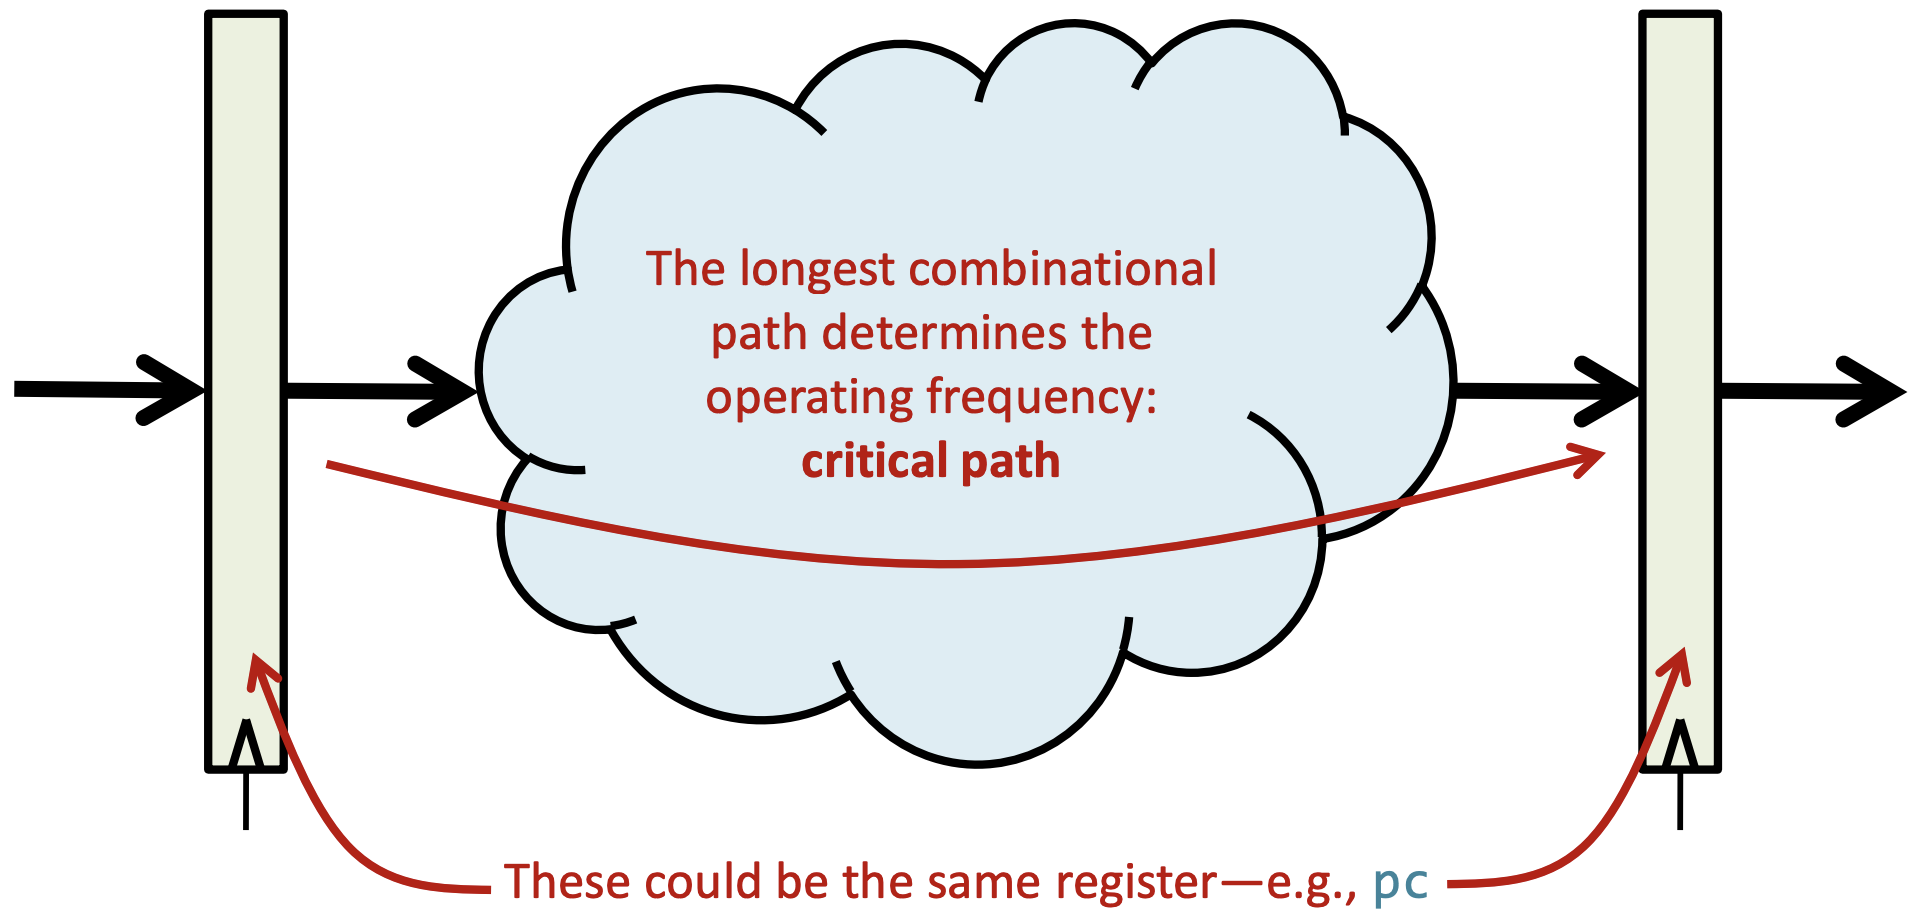
\includegraphics[width=0.45\textwidth]{chapters/chapter4b/images/prop_time.png}
    \end{center}
\end{minipage}
\hfill
\vline
\hfill
\begin{minipage}[htp]{0.45\textwidth}
    \begin{center}
        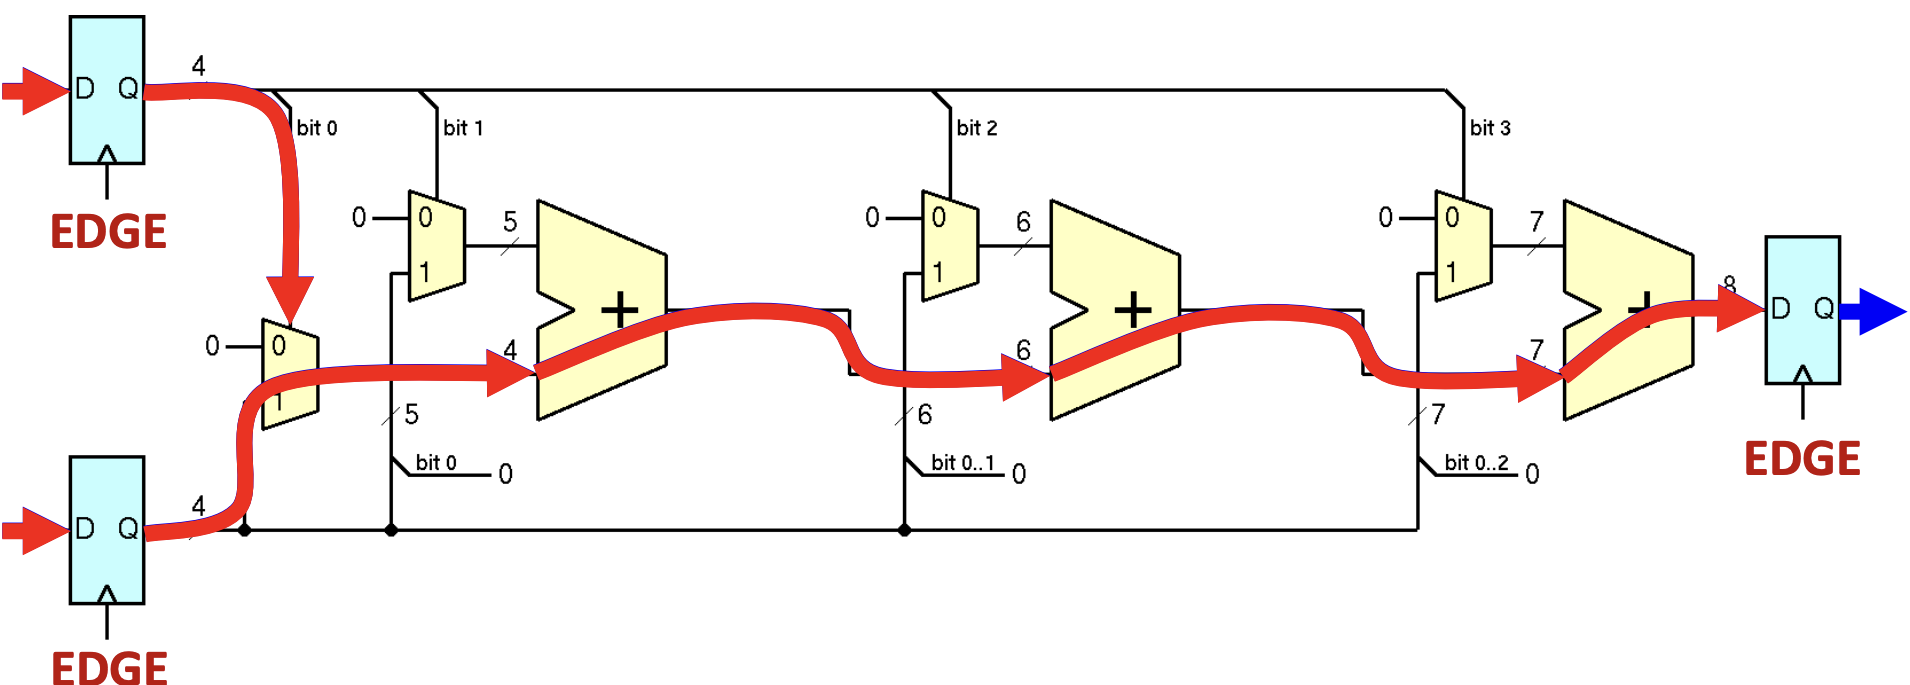
\includegraphics[width=0.65\textwidth]{chapters/chapter4b/images/prop_diag.png}
    \end{center}
\end{minipage}
To guarantee reliable operation, the \texttt{clock} period must be at least as long as the circuit's \textbf{critical path delay}—the longest delay through the combinational logic. This ensures that all signal transitions complete before the next clock edge arrives.

\[
\texttt{Clock Period} \geq \texttt{Critical Path Delay}
\]
\[
T_{\texttt{clock}} \geq T_{\texttt{critical\_path}}
\]


\noindent \textbf{Example:} In the circuit shown, the critical path is highlighted, indicating the longest combinational delay that dictates the minimum \texttt{clock} period.

\newpage

\subsubsection{Adding Intermediate Registers}
\textbf{Intermediate Registers} can be added to break up the critical path into smaller segments, reducing the overall delay. This technique is known as \textbf{pipelining}.
\begin{center}
    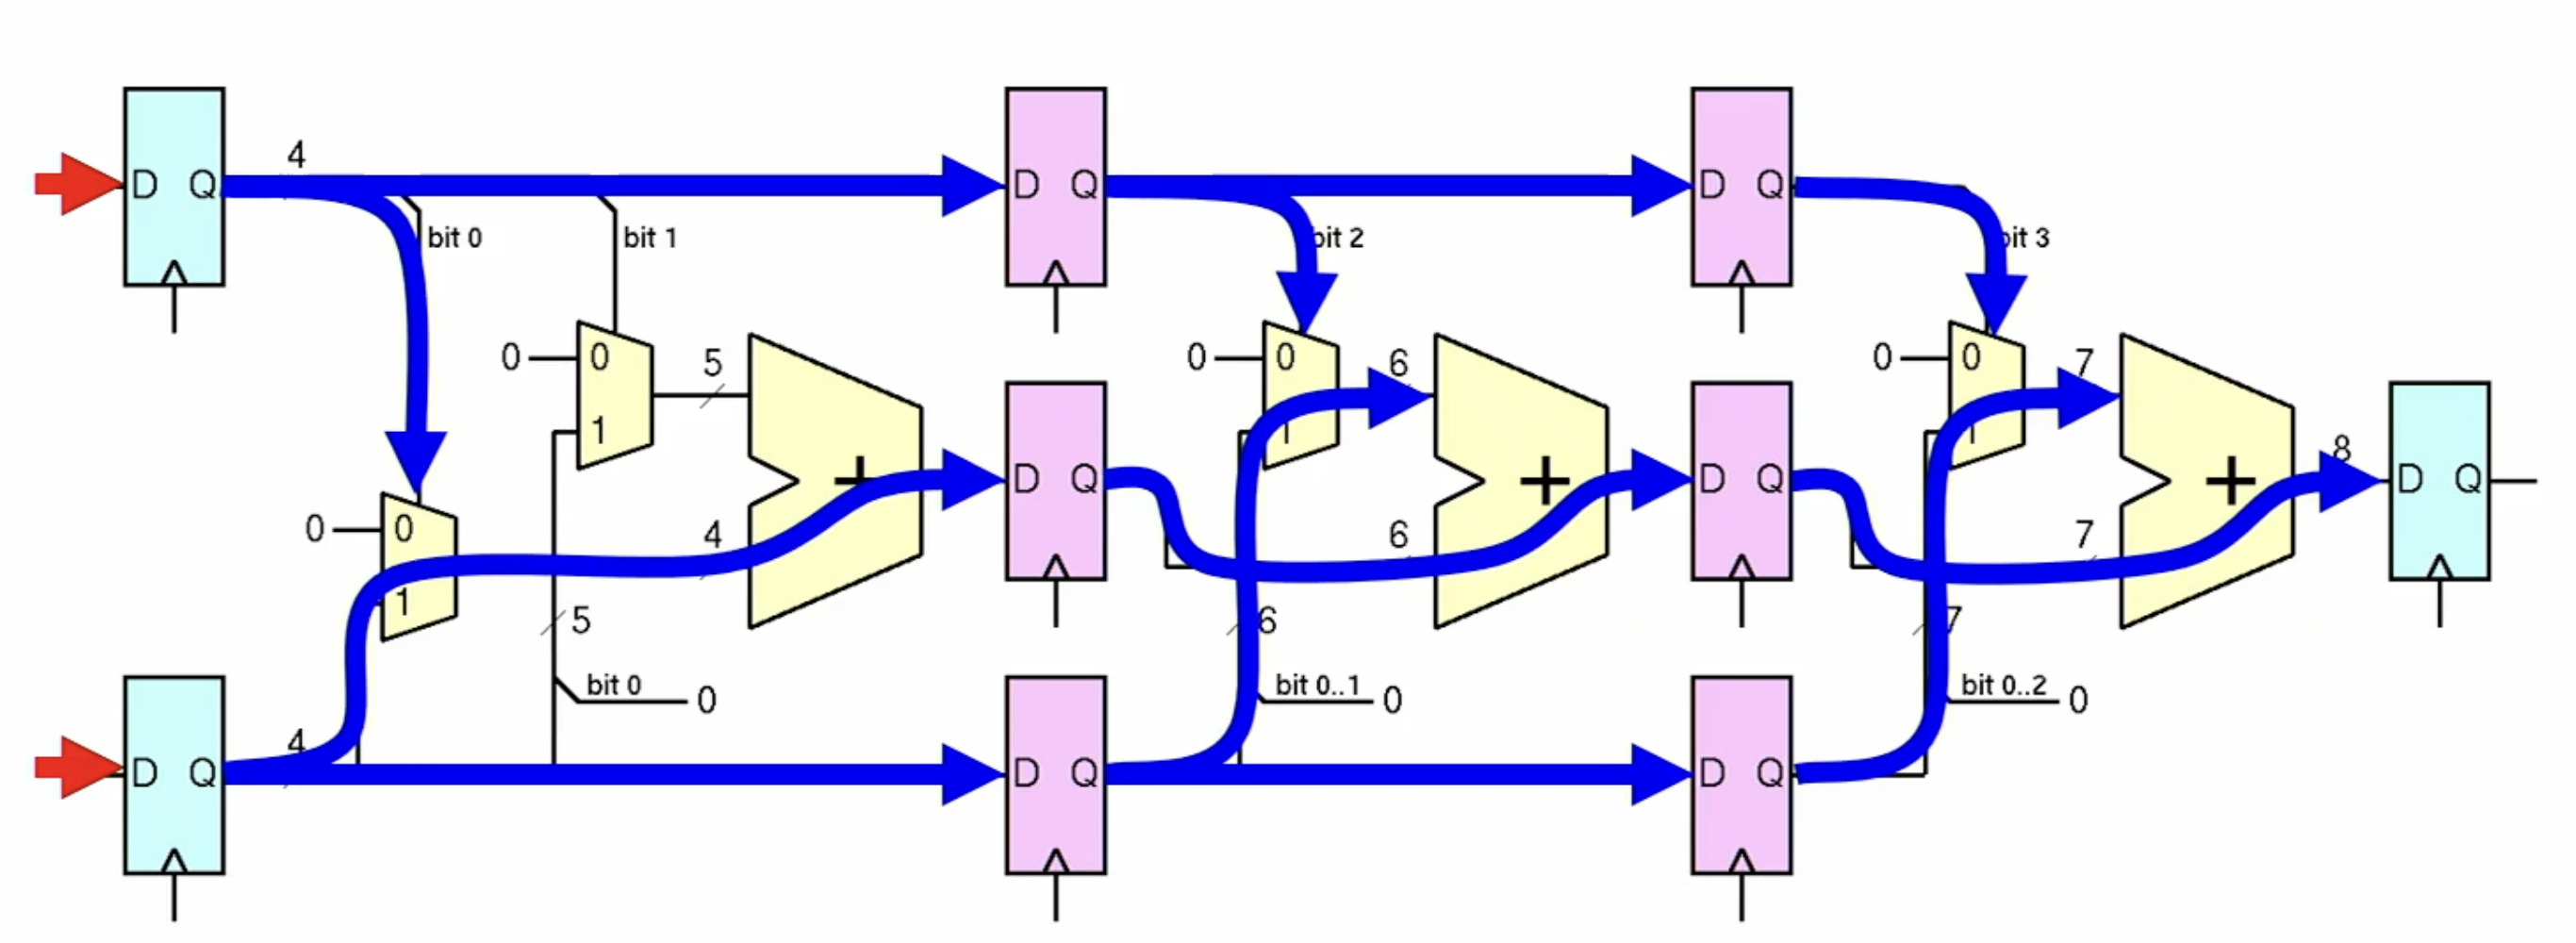
\includegraphics[width=0.65\textwidth]{chapters/chapter4b/images/prop_pipe.png}
\end{center}
\textit{Here for example, we've divided our overall critical path into three smaller segments such that, on the first clock edge, the first segment is processed, and on the second clock edge, the second segment is processed, and so on.}
Now, this new circuit has a shorter critical path, allowing for a faster clock period.
$$T_{\texttt{clock, pipe}} \geq T_{\texttt{new\_critical\_path}} \approx \frac{T_{\texttt{critical\_path}}}{3}$$
While this makes clock periods shorter, it also increases the number of clock cycles required to complete the operation.

\noindent \textbf{Conclusion} \\
The system's functionality remains unchanged, but the clock can run N times faster due to reduced critical path length from intermediate registers, at the cost of requiring N cycles to compute results. This allows for a finer control over the system.

\subsection{Pipelining: Enhancing System Throughput}

Pipelining is a technique widely used in computer architecture to improve the throughput of a system by overlapping the execution of multiple operations. It achieves this by dividing a task into smaller stages, where each stage performs a portion of the overall operation. These stages are connected in a pipeline structure, allowing multiple operations to be processed simultaneously.

\subsubsection*{How Pipelining Works}
A pipeline is divided into distinct stages, each designed to execute a specific part of the operation. For example, in an arithmetic operation, the stages might include fetching data, decoding instructions, performing calculations, and writing results. Each stage operates independently and processes data sequentially.

To understand this, consider a factory analogy where a product goes through three steps:
\begin{itemize}
    \item[] \textbf{Step 1:} Assembly
    \item[] \textbf{Step 2:} Painting
    \item[] \textbf{Step 3:} Packaging
\end{itemize}

In a \textbf{non-pipelined factory}, one worker completes all three steps for one product before starting the next. If each step takes 1 minute, three products would require \( 3 \times 3 = 9 \) minutes.

\hspace{-10px}
\begin{center}
    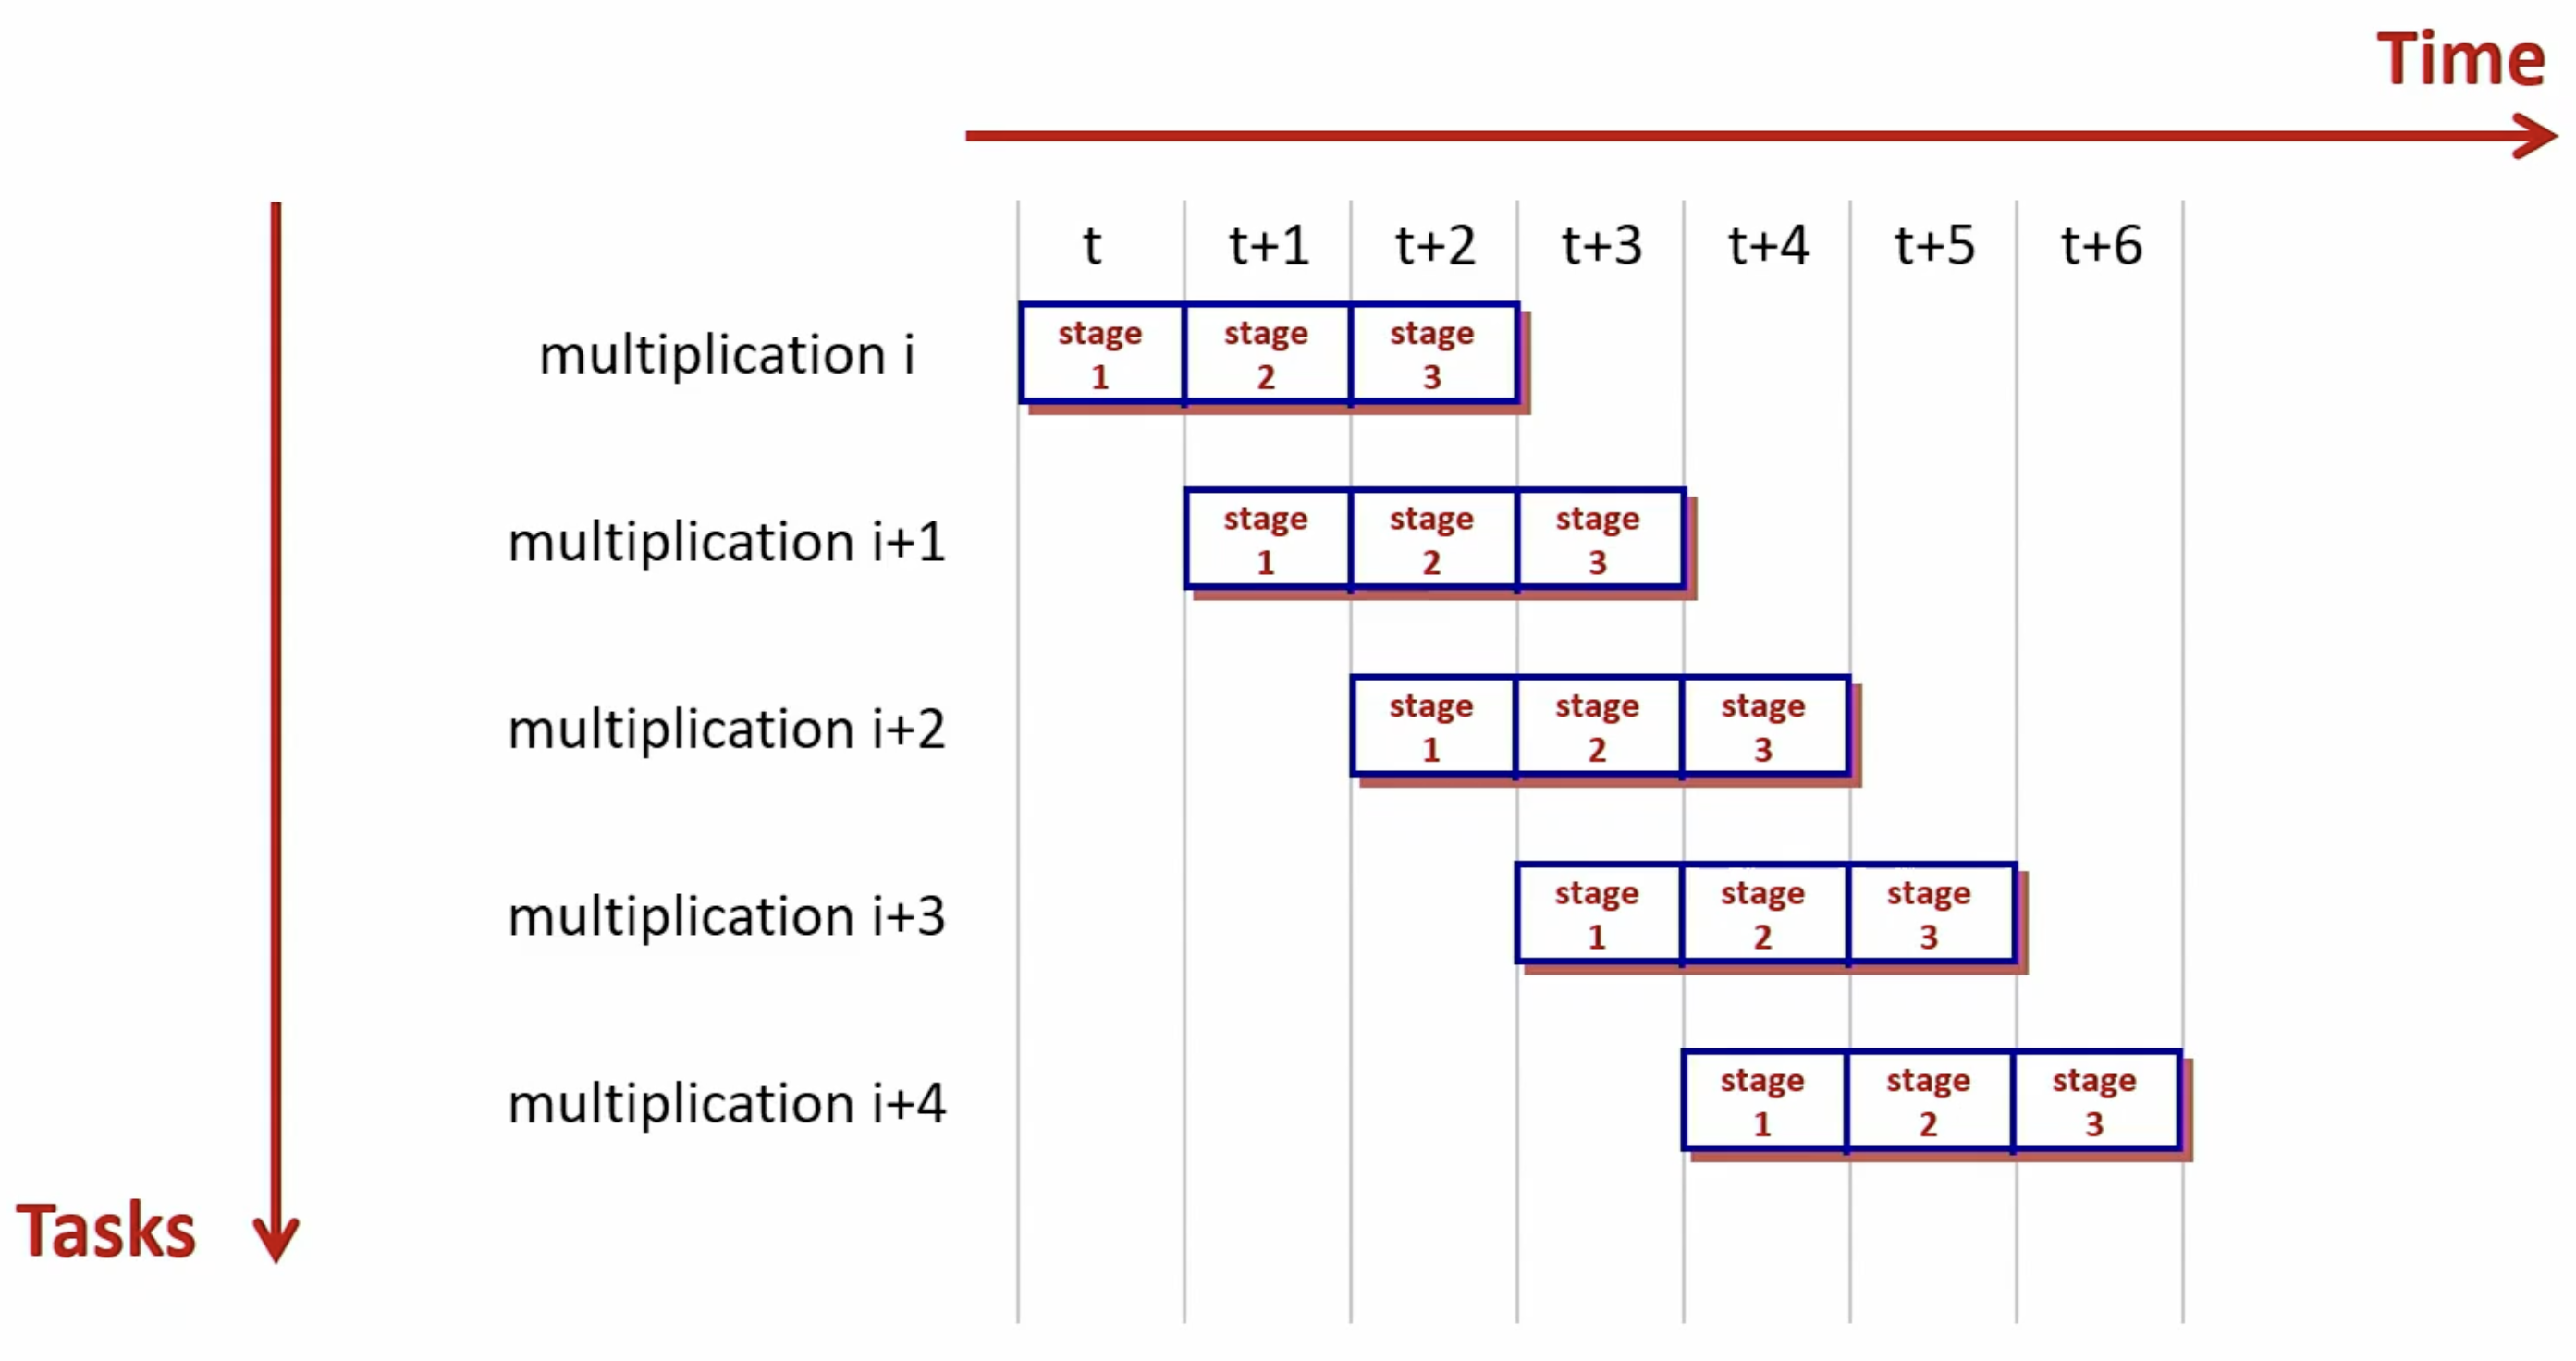
\includegraphics[width=0.65\textwidth]{chapters/chapter4b/images/parallel.png}
\end{center}
In a \textbf{pipelined factory}, the work is divided among three workers:
\begin{itemize}
    \item[] \textbf{At minute 1}, Worker A starts assembling the first product.
    \item[] \textbf{At minute 2}, Worker A starts assembling the second product, while Worker B paints the first.
    \item[] \textbf{At minute 3}, Worker A starts assembling the third product, Worker B paints the second, and Worker C packages the first.
\end{itemize}
By minute 5, all three products are completed, and the pipeline produces one product per minute after it is full.

This overlapping of tasks ensures that all workers are continuously busy, reducing the overall time required to produce multiple products.

\subsubsection*{Advantages of Pipelining}
The key benefits of pipelining include:
\begin{itemize}
    \item[-] \textbf{Improved Throughput:} By overlapping tasks, the system produces results at a faster rate. For instance, once the pipeline is full, one result can be produced per cycle.
    \item[-] \textbf{Efficient Resource Utilization:} Each stage works concurrently on different parts of separate operations, preventing idle resources.
    \item[-] \textbf{Scalability:} Pipelining can accommodate larger workloads by increasing the number of stages, enabling more operations to be processed simultaneously.
\end{itemize}

\subsection{Latency and Throughput}
\noindent \textbf{Latency} \\
Latency refers to the time between the start of a computation and when the result becomes available. It is given by:
\begin{itemize}
    \item \textbf{Original Circuit:} \( T \)
    \item \textbf{Pipelined Circuit:} \( \frac{T}{N} \times N = T \)
\end{itemize}

\noindent \textbf{Throughput} \\
Throughput represents the number of results produced per unit time. It is defined as:
\begin{itemize}
    \item \textbf{Original Circuit:} \( \frac{1}{T} = f \)
    \item \textbf{Pipelined Circuit:} \( \frac{1}{T/N} = \frac{N}{T} = N \times f \)
\end{itemize}

\subsection{Practical Pipelining: Latency and Throughput}
\subsubsection*{Stages and Timing in Pipelining}
Consider a pipeline with $N$ stages, where each stage $i$ takes a time $T_i$ to complete. The pipeline is divided by registers (denoted by red dashed lines), which ensure data is synchronized between stages.
\begin{center}
    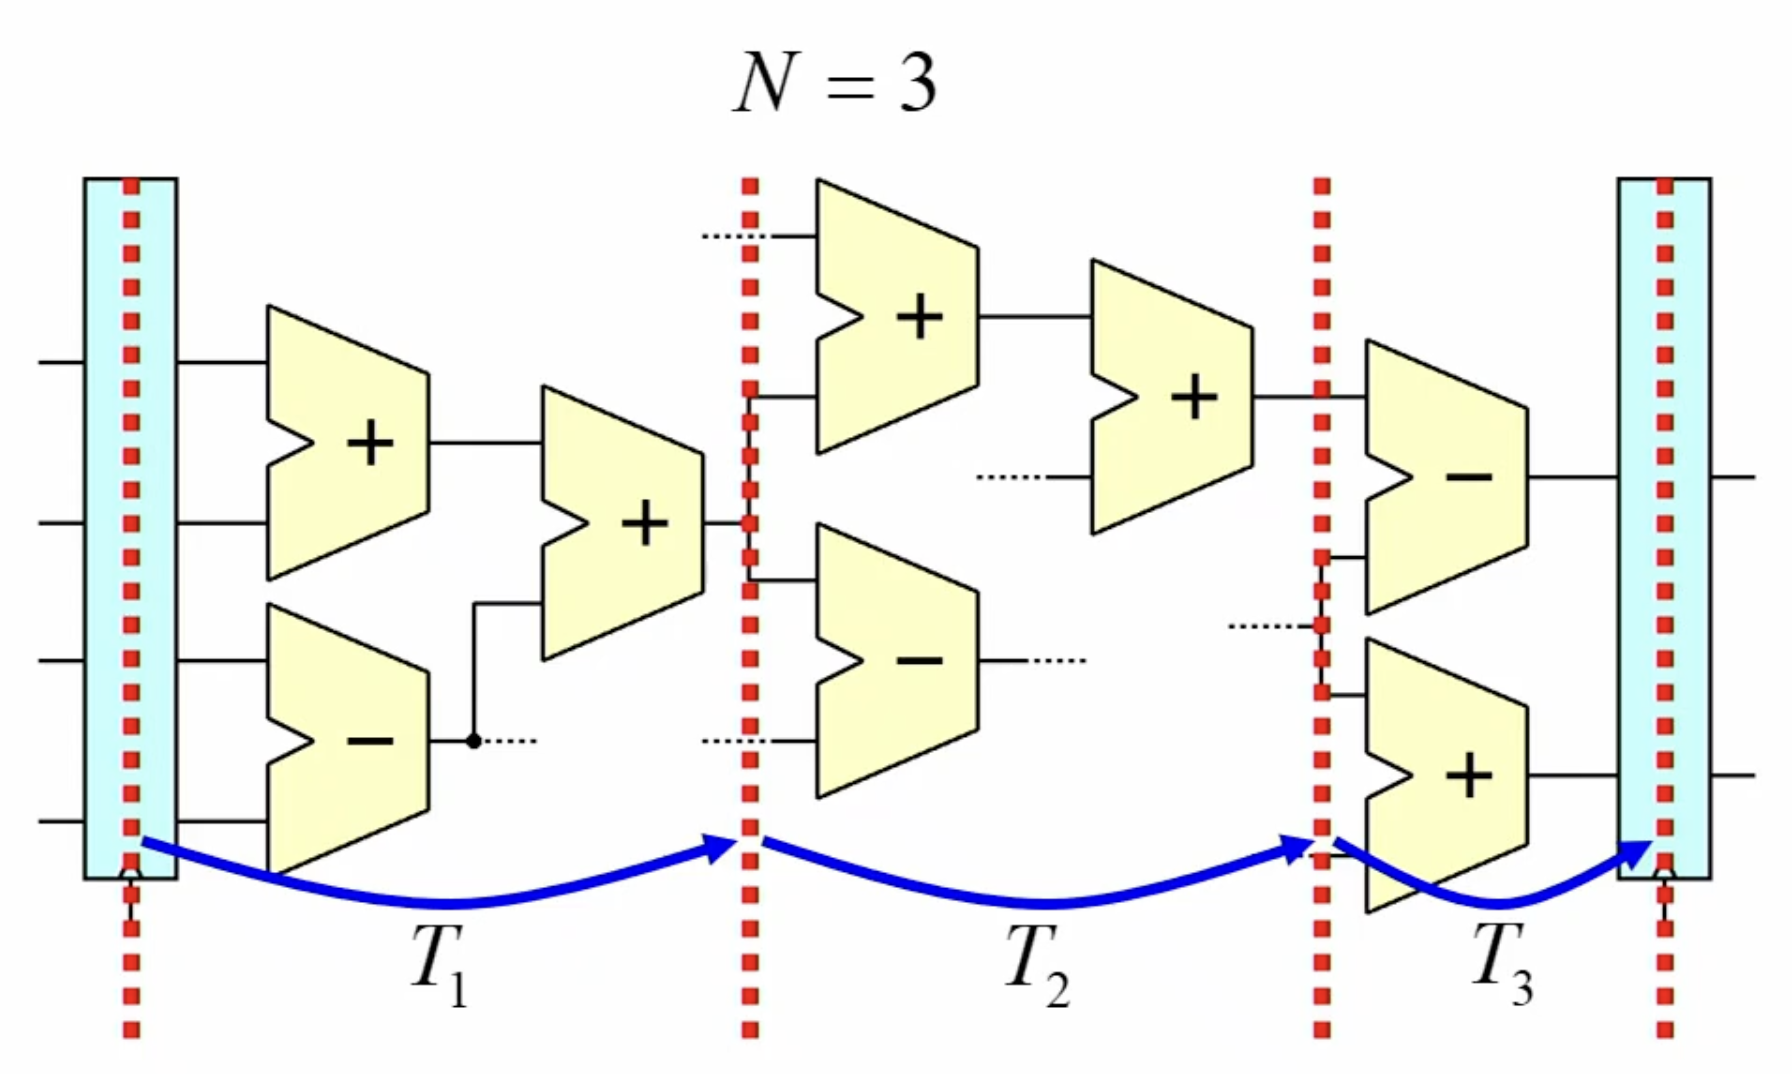
\includegraphics[width=0.45\textwidth]{chapters/chapter4b/images/practical.png}
\end{center}
The overall operation of the pipeline is governed by:
\begin{itemize}
    \item[-] \textbf{Clock Period ($T_\text{CLK,pipe}$):} This is determined by the slowest stage, $T_\text{CLK,pipe} = \max(T_i + T_\text{FF})$, where $T_\text{FF}$ accounts for flip-flop delays.
    \item[-] \textbf{Stage Timing:} Ideally, $T_i \approx T_\text{CLK,comb}/N$, where $T_\text{CLK,comb}$ is the clock period of the original non-pipelined design.
\end{itemize}

\subsubsection*{Latency and Throughput of a Pipeline}

\begin{itemize}
    \item[-] \textbf{Latency ($\lambda_\text{pipe}$):} The latency is the total time required for a single input to propagate through all $N$ stages of the pipeline. It is given by:
    \[
    \lambda_\text{pipe} = N \cdot \max(T_i + T_\text{FF}) = N \cdot T_\text{CLK,pipe}
    \]
    While pipelining increases latency compared to a non-pipelined system, the trade-off is improved throughput.

    \item[-] \textbf{Throughput ($\phi_\text{pipe}$):} Throughput measures how many operations the pipeline can complete in a given time. Once the pipeline is filled, results are produced every clock cycle. It is calculated as:
    \[
    \phi_\text{pipe} = \frac{1}{\max(T_i + T_\text{FF})} = f_\text{pipe}
    \]
    where $f_\text{pipe}$ is the pipeline operating frequency.
\end{itemize}

Pipelining is a practical approach to achieving high-speed operation in digital systems, particularly in processors and signal processing applications. By carefully designing stage timing and managing trade-offs, pipelining can achieve an optimal balance between latency and throughput.
